\documentclass[a4paper,11pt]{article}
\setlength{\topmargin}{-.5in}
\setlength{\textheight}{9in}
\setlength{\oddsidemargin}{.125in}
\setlength{\textwidth}{6.25in}
\usepackage[pdftex]{graphicx}
\usepackage{fancyvrb}

\makeatletter
\renewcommand\paragraph{%
   \@startsection{paragraph}{4}{0mm}%
      {-\baselineskip}%
      {.5\baselineskip}%
      {\normalfont\normalsize\bfseries}}
\makeatother

\begin{document}

% The Title page
\begin{titlepage}
\begin{center}

\includegraphics[width=0.6\textwidth]{fig/logo}\\[3cm]    
\textsc{\LARGE Patty / Mapping the Via Appia in 4D}\\[0.5cm]
\textsc{\large Via Appia 4D GIS: OSG Viewer Software User Manual}\\[0.5cm]
\vfill
\end{center}
{\large
\emph{O. Martinez-Rubi } \\
}
{\large
{Netherlands eScience Center, \\
Science Park 140 (Matrix 1), 1098 XG Amsterdam, the Netherlands\\
}
}
\begin{center}
{\large \today}
\end{center}
\end{titlepage}

\tableofcontents

\newpage

\section{4D Viewer API}

The \textit{launcher} tool starts the 4D viewer after the synchronization of the data is finished. Two windows are visible: one with the 4D scene and the other one with the GUI which contains four tabs. In the next Subsubsections we describe each of these tabs. By clicking on the Help button in the GUI main menu bar a more detailed help text can be displayed (only in Dutch). 

In order to load the data into the scene we need to open the XML configuration file. Click on File and Open, navigate to the folder where the data has been downloaded and select the ViaAppia.conf.xml file (the default is /Users/\textless{}UserLocal\textgreater{}/ViaAppia/DATA/OSG/ViaAppia.conf.xml).

This will load the 4D scene and some data will already be visible in the visualization window. By default only the low resolution background point cloud is visible. This data is static and can not be moved, resized or rescaled. For each site there can be different pictures, meshes and point clouds. These are active objects which are not visible by default but when they become visible they can be moved, resized and rescaled.

A very important characteristic of this GIS system is that each site is identified by its bounding cube. Within each site we can also identify objects or parts of the sites which are also defined by their bounding cubes. The bounding cubes (for a site or for the parts of a site) are also active objects, i.e. they can be moved, resized and rescaled. As the other types of active objects, they are not visible by default.

\subsection{Main tab}

After loading the configuration file the the main tab of the GUI looks like Figure \ref{fig-guimain}. 

\begin{figure}[!ht]
\centering
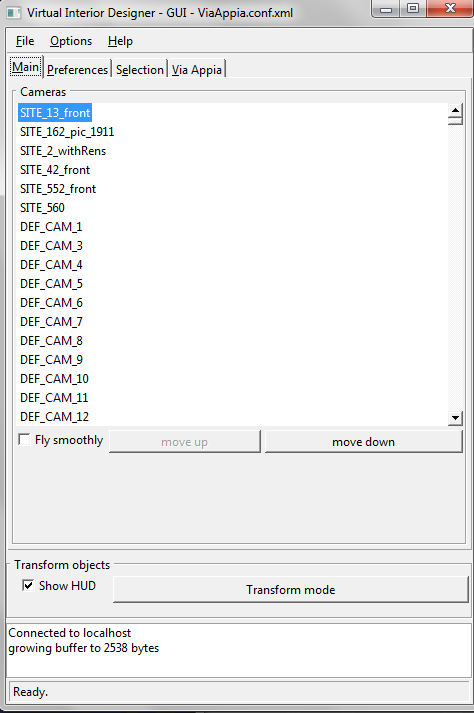
\includegraphics[scale=0.5]{fig/main}
\caption{Via Appia 4D viewer GUI: main tab}
\label{fig-guimain}
\end{figure}

This tab lists all the camera positions. The user can add new camera positions. Click on the mouse right-button on top of the cameras list and select ``Create new''. The cameras can be related to a certain site. If that is the case the camera name must start with \textit{SITE\_XXX} where \textit{XXX} is the site identifier. For the sites without user-defined camera positions a default camera position is generated based on the sites footprints.

\subsection{Preferences tab}

The preferences tab looks like Figure \ref{fig-guipref} and it has some visualization options that can be modified. The most important one is the Level of detail. Computers with low visualization resources (without powerful GPU cards) should run with lower Level of detail. Hence, if you experience a non smooth visualization try to decrease the Level of detail.

\begin{figure}[!ht]
\centering
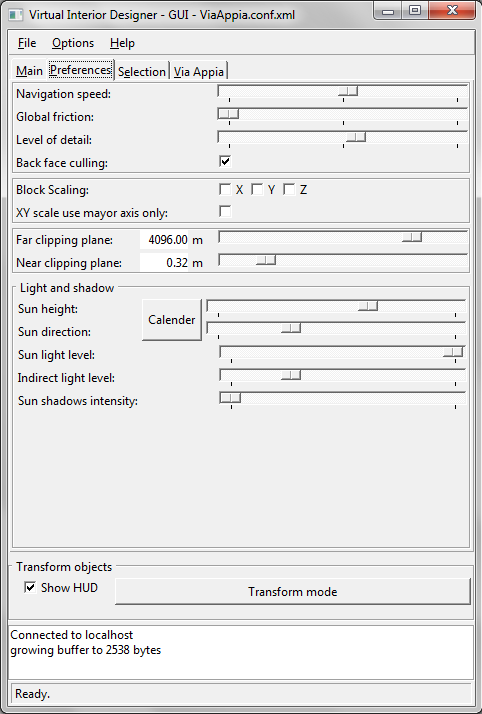
\includegraphics[scale=0.5]{fig/preferences}
\caption{Via Appia 4D viewer GUI: preferences tab}
\label{fig-guipref}
\end{figure}

The speed of the navigation is also configurable.

\subsection{Selection tab}

Clicking the ``t'' key activates the Transform mode. In this mode we can modify the position, size and rotation of active objects, i.e. points clouds, meshes and pictures related to the sites, and also their bounding cubes and bounding cubes of their parts / objects. In addition we can use the \textit{ruler} tool. Moreover we can add labels into the 4D scene and define new bounding cubes for new parts or objects within sites. See section \ref{sec:guiname} for more information about adding new labels and bounding cubes.

When you select an active object in the 4D scene, its details appear in the Selection tab as for example shown in Figure \ref{fig-guisel}. The active object can be moved, resized and rotated directly in the visualization of by specifying the values in the Selection tab (very useful when doing large changes).

\begin{figure}[!ht]
\centering
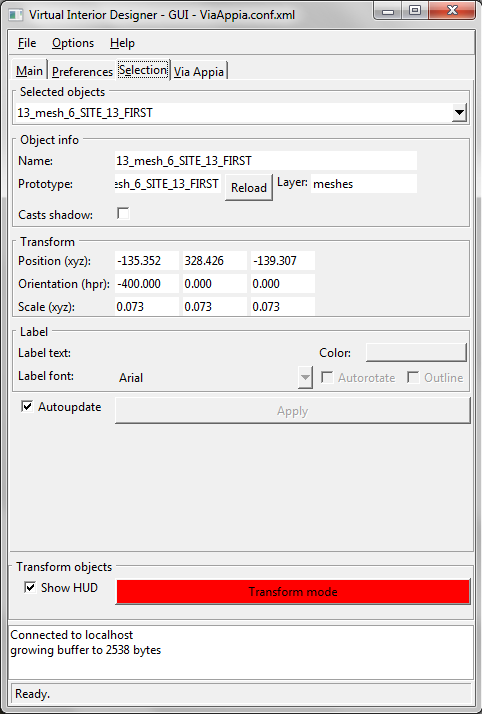
\includegraphics[scale=0.5]{fig/selection}
\caption{Via Appia 4D viewer GUI: selection tab}
\label{fig-guisel}
\end{figure}

\subsection{Via Appia tab}

\begin{figure}[!ht]
\centering
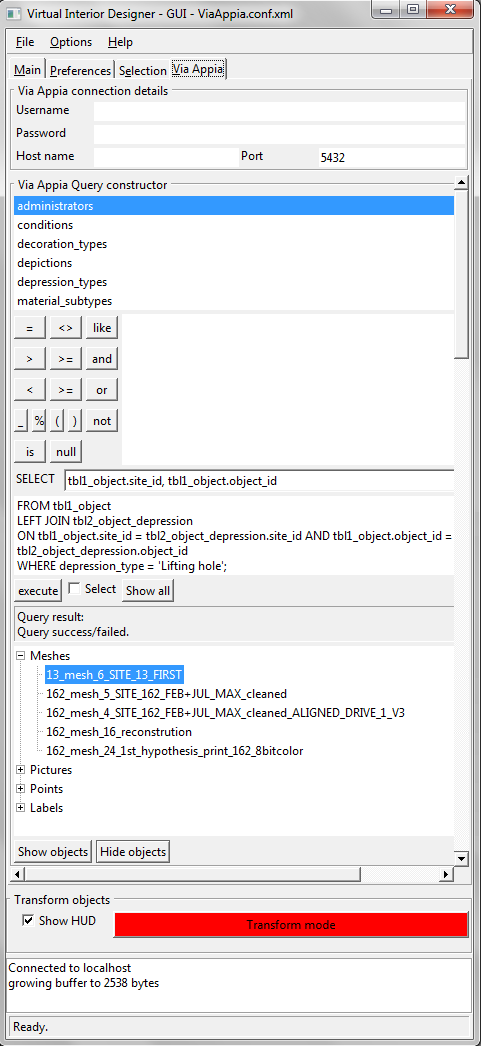
\includegraphics[scale=0.5]{fig/viaappia}
\caption{Via Appia 4D viewer GUI: Via Appia tab}
\label{fig-guiva}
\end{figure}

The last tab is called Via Appia. It is used to toggle the visibility of the different active objects. It contains two parts: 
\begin{itemize}
	\item The \textit{viaappiadb} connector. SQL statements can be constructed to access the Attributes data of the \textit{viaappiadb}. The selected columns of the SQL statement must be \textit{site\_id} or \textit{site\_id,object\_id}. After a SQL statement has been constructed and the connection details have been properly filled up it is executed in the remote DB. The bounding cubes related to the selected sites and objects (parts) will become visible in the 4D scene. If there is only one site or part selected in the DB and the \textit{select} check-box is checked in the GUI, the bounding box is selected in the 4D scene and it can be modified (see Selection tab).
	\item The active objects tree. The rest of active objects (point clouds, meshes, pictures and labels) are listed and can be showed or hidden in the 4D scene.
\end{itemize}

Note that even if different active objects become visible the user will only see them if the camera position is pointing at them. To change the camera position use the main tab.

\subsection{Naming rules}
\label{sec:guiname}

For the proper functioning of the system there are some rules that must be followed when adding new cameras, labels or bounding boxes:

\subsubsection{Cameras}

By default one camera is created per site and it is located in the center of the footprint of the site. The users can create new cameras but their names must start with \textit{SITE\_XXX} if they are related to a certain site.

\subsubsection{Labels}
 
When adding a new label the \textit{Name} (in the Object info box) must contain be \textit{*label*}. When a label is related to a site we suggest to use a name like \textit{SITE\_XXX\_label}. The \textit{Label text} (in the Label box) can contain any text.

\subsubsection{Boundings}

The different objects or parts of a site are identified by an \textit{objectId}. We consider that the site itself is a object or part of the site, in this case it is the \textit{objectId} -1. 
When adding a bounding for a new site use the ``t'' key to enable the Transform mode. Use the last option to add a bounding box and move it and rescale it to contain the site you want. The \textit{Name} (in Object info in Selection tab) must be \textit{[siteId]\_obj\_-1}.

When adding a new bounding box for a object or part of a site the \textit{Name} must be \textit{[siteId]\_obj\_[objectId]}. For example 162\_obj\_10. Please be sure that the \textit{objectId} that you choose is not being already used. To see if it is used you can use the \textit{viaappiadb} connector. For example by executing the SQL query \textit{SELECT 162,10;} (and checking the Select check-box) you can see if there is already a object defined with id 10 for the site 162. 

\subsection{Unsynchronized 4D viewer}

If you wish to start the viewer without data synchronization you can do it directly with the script in viewer/viewer/startViewer.bat. However, note that since the synchronization is deactivated this will start the viewer with probably older data and a older configuration file. In addition, in this mode the changes done in the scene are not automatically committed to the \textit{viaappiadb}. Therefore, we discourage using the viewer/viewer/startViewer.bat.

%\appendix

%\section{4D viewer XML configuration file}
%\label{sec:xmlconfig}

%\subsection{Creating a XML configuration file}

%\subsection{Updating the database with a XML configuration file}

%\section{Python scripts}
%\label{sec:python}

\end{document}

